%-*- coding: UTF-8 -*-
% 论文总结.tex
% 2020年7月第二周
\documentclass[UTF8]{ctexart}
\usepackage{graphicx}
\usepackage{float}
\usepackage{amsmath}
\usepackage{geometry}
\geometry{a4paper,centering,scale=0.8}
\usepackage[format=hang,font=small,textfont=it]{caption}
\usepackage[nottoc]{tocbibind}
\usepackage{url}
\usepackage{listings}
\usepackage{booktabs}
\usepackage{xcolor}     %高亮使用的颜色
\definecolor{commentcolor}{RGB}{85,139,78}
\definecolor{stringcolor}{RGB}{206,145,108}
\definecolor{keywordcolor}{RGB}{34,34,250}
\definecolor{backcolor}{RGB}{220,220,220}

\lstset{
 columns=fixed,       
 numbers=left,                                        % 在左侧显示行号
 numberstyle=\tiny\color{gray},                       % 设定行号格式
 frame=none,                                          % 不显示背景边框
 backgroundcolor=\color[RGB]{245,245,244},            % 设定背景颜色
 keywordstyle=\color[RGB]{40,40,255},                 % 设定关键字颜色
 numberstyle=\footnotesize\color{darkgray},           
 commentstyle=\it\color[RGB]{0,96,96},                % 设置代码注释的格式
 stringstyle=\rmfamily\slshape\color[RGB]{128,0,0},   % 设置字符串格式
 showstringspaces=false,                              % 不显示字符串中的空格
 language=c++,                                        % 设置语言
}

\newenvironment{myquote}
{\begin{quote}\kaishu\zihao{-5}}
{\end{quote}}

\newcommand\degree{^\circ}

\title{\heiti 基于网络流量聚类的综合安全策略生成}
\author{\kaishu 海华}
\date{\today}

\bibliographystyle{plain}

\newtheorem{thm}{定理}

\begin{document}
	\section{模型抽象}\label{sec:diyijie}
	\begin{equation}\label{eq:yi}
	    \begin{aligned}
		    &R_i: C_i \mapsto A_i
    	\end{aligned}
    \end{equation}
	Ci表示过滤流量包的规则条件。Ai表示满足规则后的行为结果。以防火墙策略为例,字段有协议,源IP:端口,目的IP:端口。具体来讲:C表示d维字段的区间,A表示访问结果允许还是拒绝。
	\begin{figure}[ht]
        \centering
        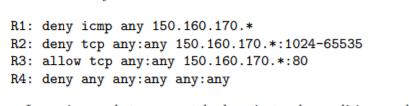
\includegraphics[scale=2.0]{picture/001.png}
        \caption{防火墙}
        \label{fig:001}
    \end{figure}
	\begin{equation}\label{eq:er}
	    \begin{aligned}
		    &C \equiv [S_c1,E_c1] [S_c2,E_c2] [S_c3,E_c3] \cdots[S_cd,E_cd] \\ &A \in \{accept,deny\}
		\end{aligned}
    \end{equation}
	\clearpage
	\section{流量聚类}\label{sec:dierjie}
	对应的聚类规则:
		\begin{itemize}
		\item[1] 每个规则对应的是一个超矩形,因为每个包的每个字段都是一个区间段
		\item[2] 相似字段的包属于同一个策略规则
		\item[3] 规则的匹配顺序基于策略生成架构
		\end{itemize}
	采用层次聚类算法对包进行聚类(Agglomerative Clutsering 是一种自底而上的层次聚类方法,它能够根据指定的相似度或距离定义计算出类之间的距离。)

	\clearpage
	\section{聚类之间距离的测量}\label{sec:disanjie}
	\begin{figure}[ht]
        \centering
        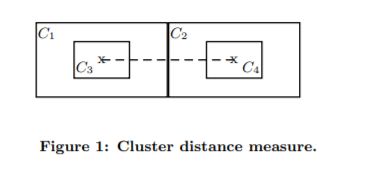
\includegraphics[scale=2.0]{picture/002.png}
        \caption{距离}
        \label{fig:002}
    \end{figure}
    \begin{figure}[ht]
        \centering
        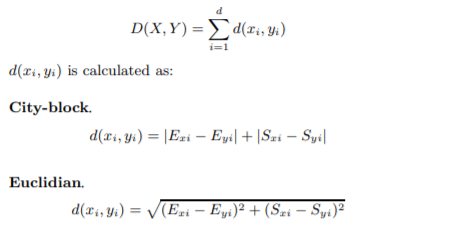
\includegraphics[scale=2.0]{picture/003.png}
        \caption{距离公式}
        \label{fig:003}
    \end{figure}
	\clearpage
	\section{策略生成的过程}\label{sec:disijie}
	\subsection{第一阶段}
	算法解析:
	\begin{itemize}
		\item[1] 初始化聚类参数
		\item[2] 将流量包p插入到距离最近的聚类Cm中
		\item[3] 如果Cm的面积大于φ,则新建另外的一个Cr
		\item[4] 否则的话,判断Cm的密度是否大于W则进行split
		\item[5] 最后判断整个C的数量,如果C的数据大于N,则合并距离最小的两个聚类,直到满足聚类数小于N的要求
	\end{itemize}
    \begin{figure}[ht]
        \centering
        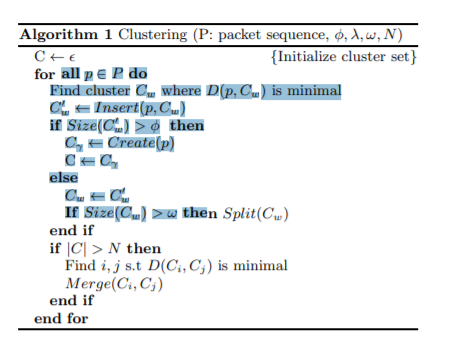
\includegraphics[scale=2.0]{picture/004.png}
        \caption{第一阶段算法}
        \label{fig:004}
    \end{figure}
	\subsection{第二阶段}
	算法解析:
	\begin{itemize}
		\item[1] 层次聚类算法中,每一层的聚类数为上一层的一半。对应while算法中的while循环,删除待合并的Ci和Cj,增加合并后的聚类。
		\item[2] ρ表示合并的时候的action比率。
	\end{itemize}
	\begin{figure}[ht]
        \centering
        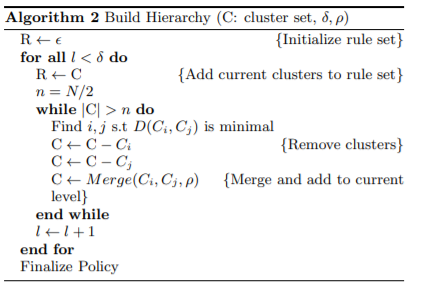
\includegraphics[scale=2.0]{picture/005.png}
        \caption{第二阶段算法}
        \label{fig:005}
    \end{figure}
	\clearpage
	\section{实验和评估}\label{sec:diwujie}
	分析了流量包中的协议,然后从协议分布、具体规则生成进行了实验验证。
	\clearpage
    \bibliography{test}
\end{document}

